\section{Frequentist analysis}\label{sec:freq}

\subsection{Hypotheses and test statistic}
We test $H_0$ (noise only) against $H_1$ (noise plus a sine-Gaussian burst). For a window with whitened bins $X$ and a unit-norm complex template $T(t_0,f_0,Q)$ the signal is $a\,T$ with $a=a_c+ia_s$ complex (amplitude and phase),
and $\ln\mathcal L=-\tfrac12\|X-aT\|^2$ up to constants. Maximising analytically over $a$ gives the likelihood-ratio statistic
\begin{equation}
\lambda(t_0,f_0,Q)=-2\ln\frac{\mathcal L(0)}{\mathcal L(\hat a)}=\rho^2(t_0,f_0,Q)=\Big|\sum_kX_kT_k^*e^{2\pi ikt_0}\Big|^2 ,\qquad
\lmax=\max_{t_0,f_0,Q}\rho^2 ,
\end{equation}
evaluated for a bank of 160 templates (40 log-spaced $f_0\in[40,450]$\,Hz $\times$ $Q\in\{3,6,10,16\}$) and for all $t_0\in[0.15,0.85]$\,s (the time shift by one FFT).
At a \emph{fixed} template Wilks' theorem~\cite{Wilks} applies: $\lambda\sim\chi^2_2$ under $H_0$ (two degrees of freedom: the two quadratures). For $\lmax$ it does not: $(t_0,f_0,Q)$ exist only under $H_1$, which is Davies' problem~\cite{Davies} and the
look-elsewhere effect. Two other statistics are used for comparison: the \emph{oracle}, $|z|^2$ at the true parameters (the Neyman--Pearson optimal test of a simple hypothesis, not available in practice), and an
\emph{excess-power} statistic~\cite{ExcessPower}, the maximum over time and over five durations (10--200\,ms) of the z-scored band energy, which assumes nothing about the morphology.

\subsection{Background: Wilks, trials factor and real noise}
Scanning $20\,000$ windows of ideal Gaussian noise, $\lmax$ is accurately described by $N_{\rm eff}=6.8\times10^3$ independent $\chi^2_2$ trials, $P(\lmax>x)=1-(1-e^{-x/2})^{N_{\rm eff}}$:
a single-template threshold of $\lambda\approx9$ at FAP $10^{-2}$ becomes $\approx27$ for the bank. On real noise (Fig.~\ref{fig:bkg}) the distribution follows the Gaussian one up to $\lmax\approx22$ and then leaves it, developing a nearly flat \emph{floor} at
a few $10^{-3}$ per window: the glitches of Section~\ref{sec:data}. The thresholds set on the training chunks are $33.6$ (FAP $10^{-2}$) and $114$ (FAP $10^{-3}$), against $\approx27$ and $\approx31$ for Gaussian noise
with the same trials factor. Epochs differ enormously: $\sim10\,\%$ of the windows of chunk~2 exceed $\lmax=60$, and this chunk drives the training threshold.

\begin{figure}[h]\centering
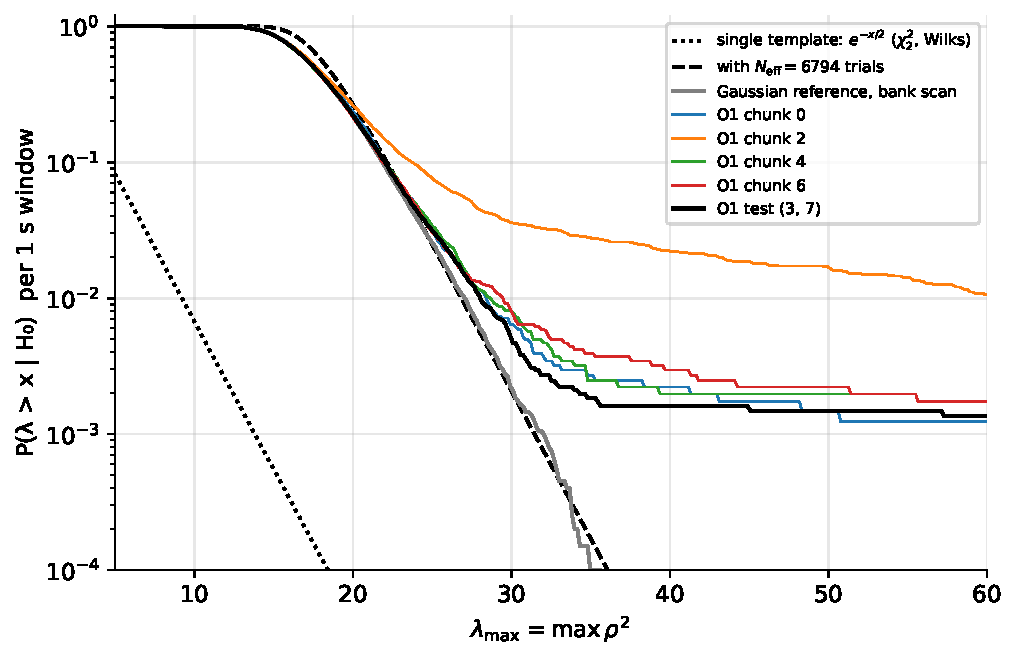
\includegraphics[width=0.62\textwidth]{fig03_background.pdf}
\caption{Survival function of $\lmax$ under $H_0$: single-template $\chi^2_2$ (dotted), $\chi^2_2$ with $N_{\rm eff}=6794$ trials (dashed), Gaussian simulation (grey), real chunks (colours) and test chunks (black).}\label{fig:bkg}
\end{figure}

\subsection{Calibration on unseen epochs}
The threshold at false-alarm probability $\alpha$ is the $(1-\alpha)$ quantile of the training background. On the test chunks the observed FAP of the bank is $2.2\times10^{-3}$ for $\alpha=10^{-2}$ (68\,\% interval $1.7$--$2.9\times10^{-3}$)
and $1.2\times10^{-3}$ for $\alpha=10^{-3}$; the excess-power statistic gives $3.7\times10^{-3}$ and $1.1\times10^{-3}$. The thresholds are therefore \emph{conservative}, by a factor $\approx4.5$ at $10^{-2}$, because the glitchy chunk~2
inflates the training background. The false-alarm probability is not a property of the statistic but of the (non-stationary) background it is calibrated on; a threshold transferred to another epoch can be off by a factor of several in either direction.

\subsection{Efficiency and ROC}
For each morphology and SNR, $500$ bursts are injected in randomly chosen test windows (with the PSD of their own chunk) and the fraction above threshold is the efficiency (Fig.~\ref{fig:eff}, Table~\ref{tab:eff}).
\begin{itemize}[nosep]
\item \textbf{Sine-Gaussian.} The oracle reaches 50\,\% efficiency at $\snr=3.0$ and 90\,\% at $4.4$; the bank at $5.5$ and $6.9$; excess power at $6.8$ and $9.7$. The oracle--bank gap is the price of not knowing $(t_0,f_0,Q)$ (look-elsewhere);
the bank--excess-power gap is the price of not using the signal shape.
\item \textbf{Pulse and chirp.} Outside the template family the bank is mismatched but still better than the agnostic statistic: the Gaussian pulse is well covered by low-frequency, low-$Q$ templates ($\snr_{50}=5.9$ against $6.1$), and the chirp loses
only $1.7$ in $\snr_{50}$ with respect to the sine-Gaussian ($7.2$) while excess power needs $10.8$.
\item \textbf{FAP $10^{-3}$.} Because of the glitch floor, lowering the FAP tenfold costs much more than in Gaussian noise: with the training-background threshold the 50\,\% point of the bank moves from $\snr\approx5.5$ to $\approx11$ (dotted curves); with the validation background, a cleaner epoch set, it moves from $4.9$ to $6.8$ (sine-Gaussian, Section~\ref{sec:threshconv}): most of the cost is the glitchy chunk~2 of the training set, i.e.\ a property of the epoch.
\end{itemize}
The ROC AUC at $\snr=8$ is $0.997/0.971$ (bank/excess power) for sine-Gaussians, $0.995/0.994$ for pulses and $0.983/0.820$ for chirps.

\begin{figure}[h]\centering
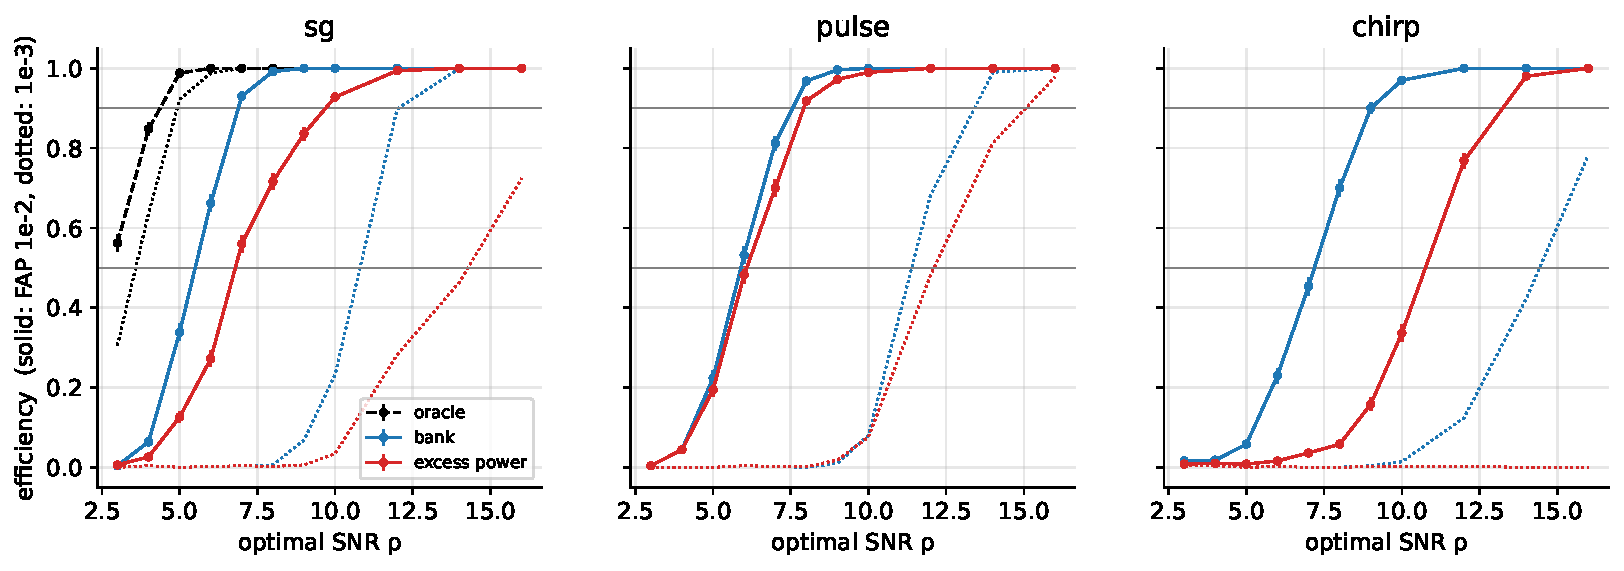
\includegraphics[width=0.95\textwidth]{fig03_efficiency.pdf}
\caption{Efficiency against optimal SNR at FAP $10^{-2}$ (solid, with binomial errors) and $10^{-3}$ (dotted) for the three morphologies: oracle (black, sine-Gaussian only), bank (blue), excess power (red).}\label{fig:eff}
\end{figure}

\begin{table}[h]\centering\small
\begin{tabular}{llrrrr}
\toprule
morphology & statistic & $\snr_{50}$ & $\pm$ & $\snr_{90}$ & $\pm$\\
\midrule
sine-Gaussian & oracle & 3.00 & 0.00 & 4.37 & 0.09\\
 & bank & 5.50 & 0.07 & 6.89 & 0.05\\
 & excess power & 6.79 & 0.08 & 9.70 & 0.14\\
Gaussian pulse & bank & 5.90 & 0.07 & 7.56 & 0.08\\
 & excess power & 6.08 & 0.10 & 7.92 & 0.06\\
linear chirp & bank & 7.19 & 0.09 & 9.00 & 0.12\\
 & excess power & 10.76 & 0.09 & 13.25 & 0.10\\
\bottomrule
\end{tabular}
\caption{Optimal SNR at which the efficiency reaches 50\,\% and 90\,\% (FAP $10^{-2}$, test chunks).}\label{tab:eff}
\end{table}

\subsection{Maximum-likelihood parameter estimation}
For detected sine-Gaussians the bank maximum is refined with \texttt{iminuit} on the continuous profile $\rho^2(t_0,f_0,Q)$ and the covariance of the MLE is compared with the Fisher (Cram\'er--Rao) matrix, obtained from the Hessian of $-\rho^2$ at the truth on noise-free data,
$\mathrm{cov}=2[\nabla^2(-\rho^2)]^{-1}$. With $300$ injections per SNR (Fig.~\ref{fig:pe}) the MLE saturates the bound for $\snr\gtrsim10$ ($f_0$: RMS $2.8$ against $2.7$\,Hz at $\snr=10$; $0.90$ against $0.90$\,Hz at $\snr=30$) and the Hessian errors of \texttt{iminuit} agree with it.
At low SNR the RMS departs upward (at $\snr=6$ the RMS of $f_0$ is $34$\,Hz against $4.5$ predicted) because the likelihood surface has secondary maxima to which the estimate jumps; the robust width stays near the bound. This is the classical threshold effect of non-linear parameters.

\begin{figure}[h]\centering
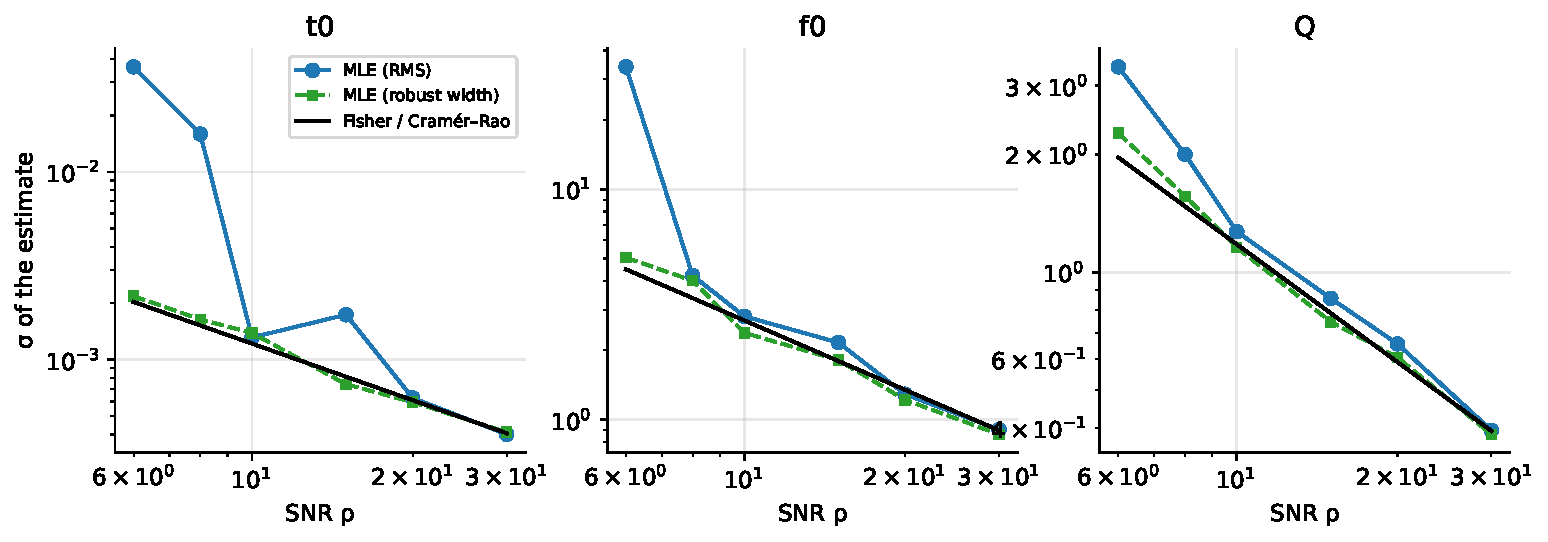
\includegraphics[width=0.85\textwidth]{fig03_pe_fisher.pdf}
\caption{Standard deviation of the MLE of $t_0$, $f_0$, $Q$ against SNR: RMS (blue), robust width (green) and Fisher/Cram\'er--Rao bound (black).}\label{fig:pe}
\end{figure}

\subsection{Toy Monte Carlo: bias, pulls and coverage}
With a known template and unknown SNR $s\ge0$ the data reduce to $z=s\,e^{i\varphi}+n$, $n\sim\mathcal N(0,I_2)$; the MLE is $\hat s=|z|$ (Rice distribution) and $-2\Delta\ln\mathcal L_p(s)=(\hat s-s)^2$, so the profile-likelihood interval is $[\hat s-1,\hat s+1]$ truncated at zero.
With $4\times10^4$ toys per value of $s$ (Fig.~\ref{fig:toy}): the MLE is biased upward at low SNR ($E[\hat s]-s=1.25$ at $s=0$, $\sqrt{\pi/2}$; $0.27$ at $s=2$; $0.05$ at $s=10$); the profile-likelihood interval covers $39\,\%$ at $s=0$ (nominal $68\,\%$), overshoots to $\approx74\,\%$ near $s=1$ and is within one per cent of $68\,\%$ only for $s\gtrsim3$ (parameter on the boundary: Wilks' regularity fails);
the Neyman central and Feldman--Cousins belts~\cite{FeldmanCousins} cover $68.3\,\%$ at every $s$ by construction. The same experiment repeated with a fixed template injected in $5000$ real windows per SNR gives the same bias, RMS and coverage within $0.03$, so the single-template amplitude estimate is insensitive to the glitches
(whereas the bank statistic of the previous section is not).

\begin{figure}[h]\centering
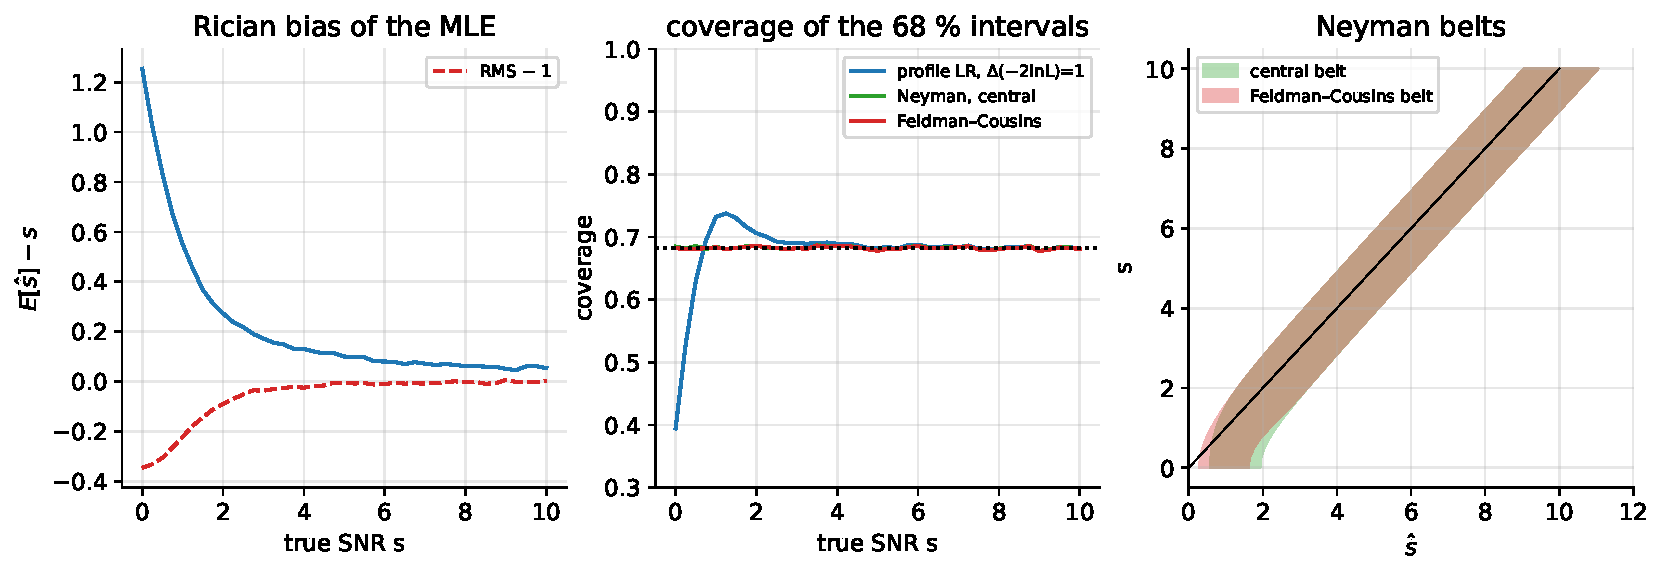
\includegraphics[width=0.95\textwidth]{fig03_toys_amplitude.pdf}
\caption{Toy Monte Carlo of the amplitude estimate. Left: bias and $\mathrm{RMS}-1$ of $\hat s$. Centre: coverage of the 68\,\% profile-likelihood, central Neyman and Feldman--Cousins intervals. Right: the two Neyman belts.}\label{fig:toy}
\end{figure}

\subsection{Systematic study}
The observable is the sine-Gaussian efficiency $\varepsilon(\snr=8)$ at FAP $10^{-2}$; each variant changes one analysis choice and recomputes the whole chain on the \emph{same} windows and injections, so that differences are correlated.
Barlow's criterion~\cite{Barlow} (a variation is significant if $|\Delta|/\sigma_\Delta>2$, $\sigma_\Delta^2=|\sigma_{\rm var}^2-\sigma_{\rm nom}^2|$) gives Table~\ref{tab:sys}.
Only the use of the \emph{mean} instead of the median in the Welch average is large and unambiguous ($+0.025$): the mean PSD is inflated by glitches, lowers the whitened-noise level and the threshold ($42.9$ against $45.0$). All other variants change $\varepsilon$ by at most $0.007$ (1--3$\sigma$).
We quote $0.025$ as the systematic uncertainty on $\varepsilon(\snr=8)$.
\begin{table}[h]\centering\small
\begin{tabular}{lrrrr}
\toprule
variant & threshold & $\varepsilon$ & $\Delta$ & $|\Delta|/\sigma_\Delta$ (Barlow)\\
\midrule
nominal & 45.0 & 0.928 & -- & --\\
PSD mean-average & 42.9 & 0.953 & $+0.025$ & 5.3\\
PSD 2\,s segments & 44.6 & 0.935 & $+0.007$ & 2.8\\
PSD 8\,s segments & 44.6 & 0.933 & $+0.005$ & 2.4\\
band 20--500\,Hz & 45.0 & 0.929 & $+0.001$ & 1.1\\
band 30--400\,Hz & 45.0 & 0.925 & $-0.003$ & 1.9\\
coarse bank (20 $f_0$) & 44.0 & 0.921 & $-0.007$ & 2.9\\
\bottomrule
\end{tabular}
\caption{Systematic variants (threshold from chunks 0 and 2, efficiency from 1000 injections in chunks 3 and 7).}\label{tab:sys}
\end{table}

\subsection{Signal-consistency test and a combined ranking statistic}\label{sec:chi2}
The look-elsewhere and glitch costs of the bank can be reduced without changing the template family (notebook~16). The best template is split in $8$ frequency bands of equal power; $\chi^2=\sum_i|z_i-z/8|^2\cdot8$ measures how far the distribution of the matched-filter output over the bands departs from that of the template (Allen's $\chi^2$, $14$ degrees of freedom for Gaussian noise and an exact template), and the re-weighted SNR is $\rho/[(1+c^3)/2]^{1/6}$ for $c=\chi^2/\mathrm{dof}>1$. A logistic regression and a gradient-boosted classifier on $(\rho^2,\chi^2,\text{new SNR},\max|v|,\text{kurtosis},f_0,Q)$ are trained on the training chunks only.
\begin{table}[h]\centering\small
\begin{tabular}{lrr}
\toprule
statistic & FAP $10^{-2}$ & FAP $10^{-3}$\\
\midrule
bank $\rho^2$ & $5.51$ & $7.76$\\
bank with $\chi^2$ veto ($c\le3$) & $5.44$ & $6.35$\\
new SNR & $5.63$ & $6.72$\\
logistic regression (7 features) & $5.54$ & $6.46$\\
gradient boosting (7 features) & $5.38$ & $6.34$\\
\midrule
CNN, fresh injections (notebook~07) & $4.50$ & $5.48$\\
\bottomrule
\end{tabular}
\caption{Mean $\snr_{50}$ over sine-Gaussian, pulse and chirp (validation thresholds; bootstrap error $0.09$ at $10^{-2}$, $0.2$ at $10^{-3}$).}\label{tab:chi2}
\end{table}
At FAP $10^{-2}$ nothing changes: the bulk of the background is Gaussian. At $10^{-3}$, where the glitch tail sets the threshold, the $\chi^2$ veto alone recovers $1.4$ of the $2.2$ units that separate the bank from the CNN and the learned ranking statistics do no better than it ($6.3$--$6.5$): consistency with the template, not a richer combination, carries the gain, and a residual $\approx0.9$ remains in favour of the network. The logistic coefficients confirm that $\rho^2$ and the new SNR carry the weight and that a large $\max|v|$ lowers the score.

\subsection{Rigour of the background: epochs, local thresholds, tails and rate limits}\label{sec:bkgrigour}
Notebook~23 examines the single-detector bank statistic on all eight chunks.
\paragraph{Epoch dependence.} Setting the threshold on seven chunks and measuring the FAP in the eighth gives observed/nominal ratios of $0.30$--$0.86$ for seven chunks and $4.3$ (FAP $10^{-2}$) or $4.9$ ($10^{-3}$) for the glitchy chunk~2, which also makes the thresholds of the others conservative. The ratio is weakly related to the share of glitchy windows (Spearman $0.29$) and to the PSD level ($0.21$): the epoch effect is carried by a few chunks of loud transients, not by a smooth drift.
\paragraph{Time-local background.} Taking the threshold of each window from the windows within $\pm150$--$600\,$s of the same chunk reduces the spread of the observed FAP across chunks from $0.013$ (leave-one-chunk-out) to $0.0006$--$0.0012$; the price is a slightly lower efficiency for loud signals ($0.976$ against $0.997$ at $\snr=8$) because loud local glitches raise the neighbours' threshold, and a gain at low SNR ($0.18$ against $0.13$ at $\snr=4$, which is the usual optimistic effect of a threshold lowered in quiet stretches).
\paragraph{Tail extrapolation.} A generalised Pareto fit to the top $5\,\%$ of the pooled train+validation background ($1217$ exceedances) gives $\xi=0.91$: a tail so heavy that the extrapolated threshold at FAP $10^{-5}$ is $5700$ ($68\,\%$ bootstrap $3500$--$8800$) against $41$ for Gaussian noise with $N_{\rm eff}=6800$. It reproduces the test FAP at $10^{-3}$ ($1.2\cdot10^{-3}$ observed) but underestimates it by a factor $\approx9$ at $10^{-4}$: the empirical tail of the glitches is not a clean power law, and extrapolation beyond the resolution of the background is not safe; the time slides of Section~\ref{sec:coinc} are the defensible way to go lower.
\paragraph{Rate limits.} With the $2.25\,$h of two-detector data of notebook~14 and $62$ zero-lag triggers against $63.1$ expected, the Feldman--Cousins $90\,\%$ upper limit on the number of detectable signals is $13.0$ (against $2.3$ for zero events and no background), i.e.\ rates of $5.8$ per hour for signals of network $\snr=15$ and $14$ per hour at $\snr=10$ (using the efficiencies of notebook~14 at FAR $<10^3\,\mathrm{yr}^{-1}$): the search is too short for a physically interesting limit.
\paragraph{Rare-event Monte Carlo.} In ideal Gaussian noise the tail of $\lambda_{\max}$ can be reached by subset simulation (multilevel splitting with preconditioned Crank--Nicolson moves that leave the Gaussian law invariant; notebook~24, four independent runs of $2000$ samples per level, $p_0=0.1$). The thresholds at FAP $0.1,10^{-2},\dots,10^{-10}$ agree with the formula $1-(1-e^{-\lambda/2})^{N_{\rm eff}}$, $N_{\rm eff}=6794$, within $0.1$--$0.6$ at FAP $\ge10^{-6}$ and $\le2$ at $10^{-10}$, with run-to-run scatter of $0.1$ to $3$ (Fig.~\ref{fig:subset}): the effective-trials model of the look-elsewhere effect is correct in Gaussian noise far beyond the reach of plain Monte Carlo ($20\,000$ windows cover only $10^{-3}$), so every excess over it measured in real noise (Section~\ref{sec:bkgrigour}) is due to the noise and not to the statistic.
\begin{figure}[h]\centering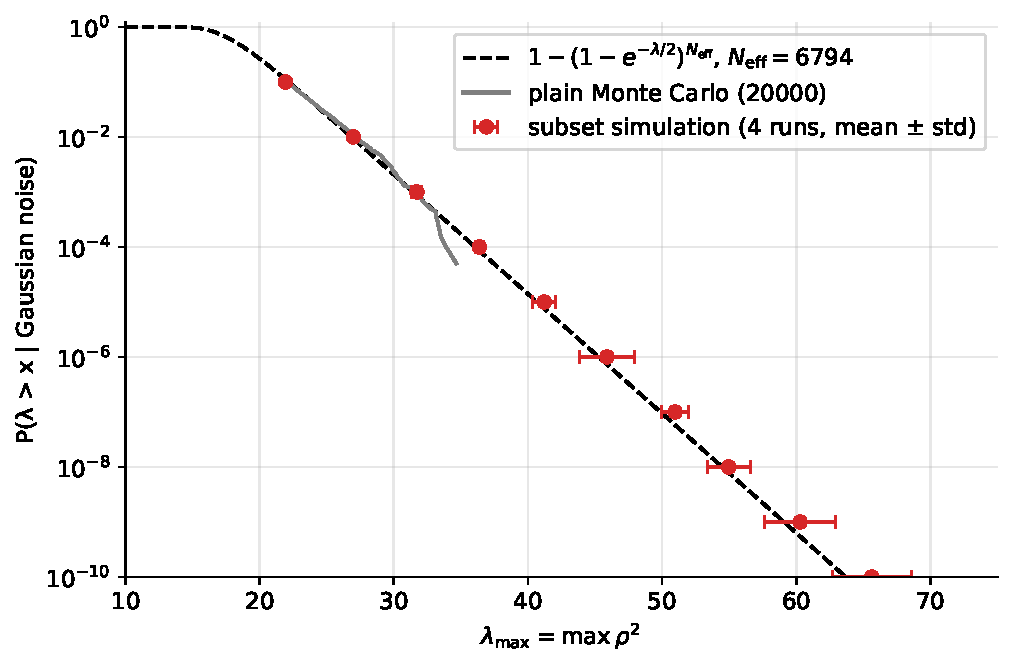
\includegraphics[width=0.6\textwidth]{fig24_subset_simulation.pdf}\caption{Gaussian-noise false-alarm probability of the bank statistic: analytic formula, plain Monte Carlo and subset simulation.}\label{fig:subset}\end{figure}

\subsection{Bank design, time-local whitening and PSD uncertainty}\label{sec:bankdesign}
Notebook~27 varies three choices of the frequentist pipeline (Fig.~\ref{fig:bankdesign}).
\paragraph{Number and placement of templates.} The fitting factor on sine-Gaussians of the project prior rises from $0.78$ ($20$ templates) to $0.91$ ($40$), $0.97$ ($80$), $0.985$ ($160$, the project) and $0.996$ ($640$); the mean $\snr_{50}$ at FAP $10^{-2}$ from $6.24$ to $5.80$, $5.61$, $5.57$ and $5.57$ (error $0.06$): beyond $\approx80$ templates a denser bank buys nothing, because the loss from the look-elsewhere effect balances the gain in overlap. At FAP $10^{-3}$ the differences ($8.0$--$8.5$ for $80$--$640$ templates) are within the error of $0.6$. A random placement of $40$ or $160$ templates is as good as the regular grid ($5.76$ and $5.62$ against $5.80$ and $5.57$; fitting factor $0.94$ and $0.98$). The $160$-template bank is therefore near the point of diminishing returns, and a bank of $80$ would give the same sensitivity at half the cost.
\paragraph{Time-local whitening.} Whitening each $512\,$s block with a PSD estimated from the block and its two neighbours instead of the whole chunk does not reduce the epoch dependence (leave-one-chunk-out observed/nominal FAP from $0.37$ to $4.2$ against $0.30$ to $4.3$; $\snr_{50}$ $5.5$/$7.9$ against $5.5$/$7.7$ at $10^{-2}$/$10^{-3}$): the epoch effect comes from glitches, not from a slowly varying PSD.
\paragraph{PSD uncertainty.} In synthetic Gaussian noise with the PSD of a real chunk, the FAP at the ideal threshold of $10^{-2}$ ($10^{-3}$) becomes $1.46\cdot10^{-2}$ ($2.3\cdot10^{-3}$) if the PSD is estimated on $32\,$s of data, $1.1\cdot10^{-2}$ ($2.0\cdot10^{-3}$) on $64\,$s and $0.96$--$0.86\cdot10^{-2}$ ($1.6$--$1.1\cdot10^{-3}$) on $256$--$4096\,$s: with the $4096\,$s chunks of the project the estimation noise is negligible, and a PSD from less than $\approx100\,$s would need the Student-$t$ correction of the likelihood.
\begin{figure}[h]\centering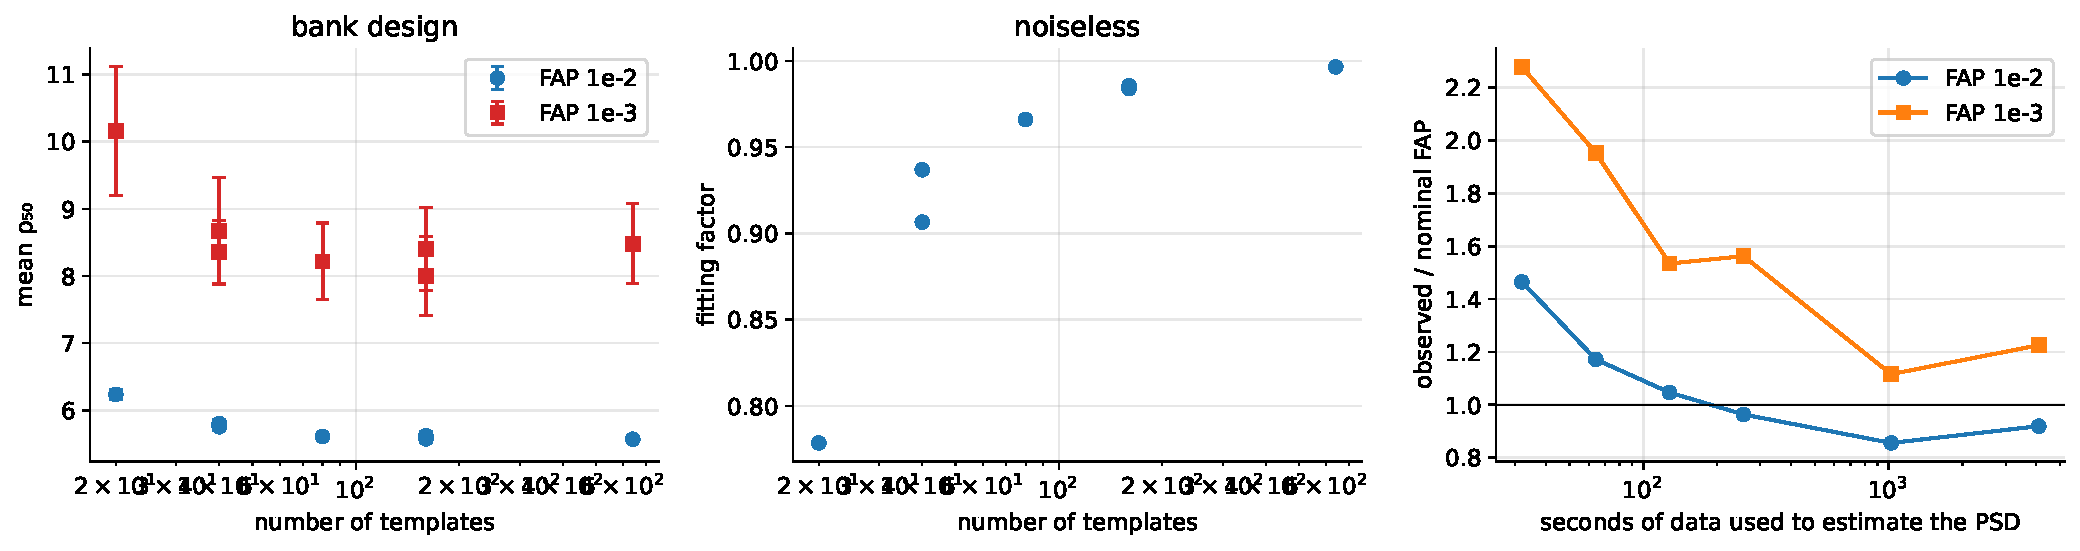
\includegraphics[width=0.98\textwidth]{fig27_bank_whitening_psd.pdf}\caption{Left: mean $\snr_{50}$ against the number of templates. Centre: fitting factor. Right: observed over nominal FAP when the PSD is estimated on $T$ seconds.}\label{fig:bankdesign}\end{figure}

\subsection{Data-quality flags}\label{sec:dq}
Notebook~35 vetoes the windows that are not entirely inside the GWOSC segments \texttt{H1\_CBC\_CAT2} (the data that remain after the category-2 vetoes; \texttt{CAT1} is identical to the science mode in our chunks). The dead time is $0.9\,\%$ overall and $7.4\,\%$ in the glitchy chunk~2 ($0$ elsewhere except $0.1\,\%$ in chunk~6), yet the flags remove $40\,\%$ of the loudest $1\,\%$ and $39\,\%$ of the loudest $0.1\,\%$ of the bank statistic (and only $4\,\%$ and $3\,\%$ of those of the CNN, which already rejects them). The leave-one-chunk-out observed/nominal FAP of the bank, $0.30$--$4.3$ at $10^{-2}$ and $0.49$--$4.9$ at $10^{-3}$ without the flag, becomes $0.76$--$1.21$ and $0.27$--$1.48$ with it; the spread across chunks drops from $0.74$ to $0.15$ (log scale) at $10^{-2}$, and the pooled threshold at FAP $10^{-3}$ from $110$ to $57$ (from $\sqrt{110}=10.5$ to $\sqrt{57}=7.5$ in the SNR of the threshold: the efficiency gain at fixed FAP, not measured here, is bounded by this). The glitch floor and the epoch dependence found in Section~\ref{sec:bkgrigour} are therefore mostly the glitches that GWOSC itself flags, and a flag-based veto should be part of any search with the template statistic; the CNN gains nothing because it never alarmed on them. The BURST flag removes less (it is a different veto set, $5$--$41\,\%$ of the top windows).
\begin{figure}[h]\centering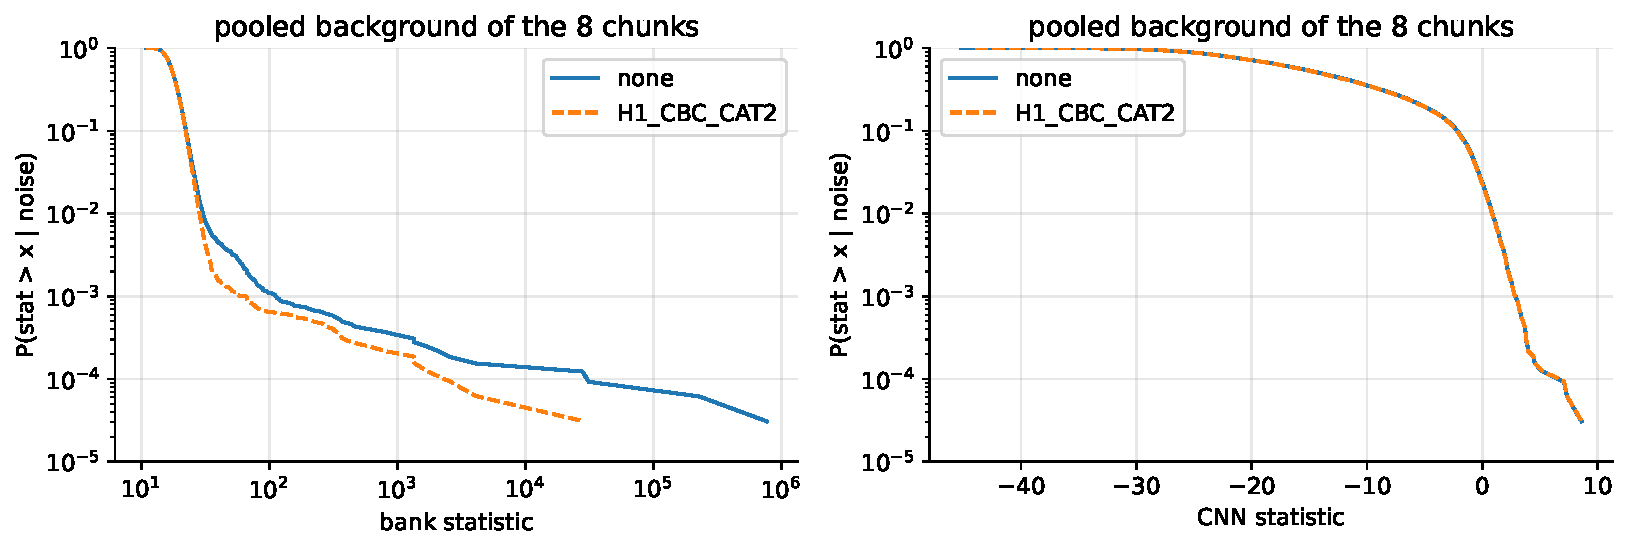
\includegraphics[width=0.98\textwidth]{fig35_dq_flags.pdf}\caption{Pooled background of the bank statistic (left) and of the CNN (right) with and without the CAT2 veto.}\label{fig:dq}\end{figure}
